\documentclass[tikz,border=4pt]{standalone}
\usepackage{times}
\usepackage{xcolor}
\usepackage{tikz}
\usetikzlibrary{arrows.meta,positioning}

\begin{document}
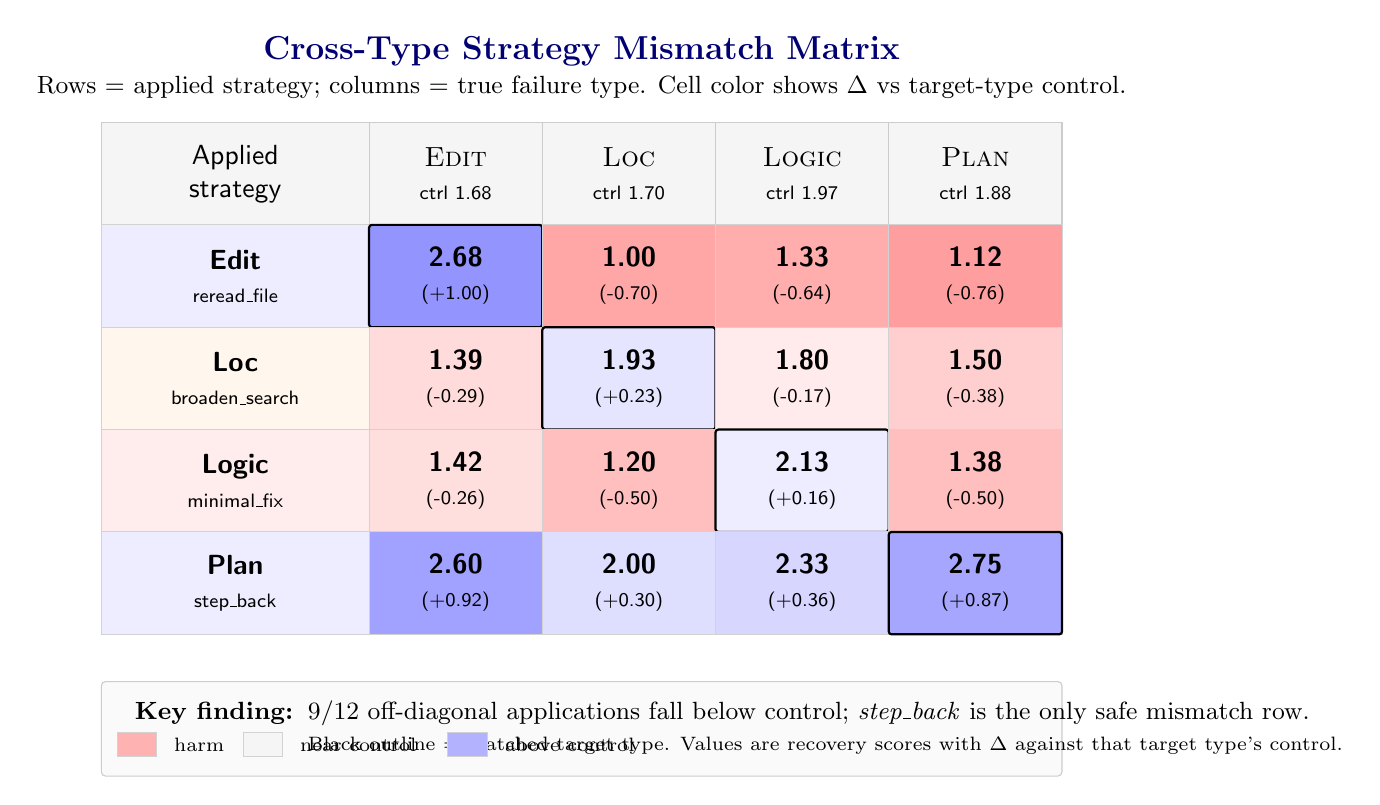
\begin{tikzpicture}[
  x=1mm,
  y=1mm,
  every node/.style={font=\sffamily},
  cell/.style={draw=gray!35, line width=0.35pt, minimum width=22mm, minimum height=13mm, align=center},
  rowlab/.style={draw=gray!35, line width=0.35pt, minimum width=34mm, minimum height=13mm, align=center},
  head/.style={draw=gray!40, fill=gray!8, line width=0.4pt, align=center},
]

% Geometry.
\def\x0{0}
\def\y0{0}
\def\roww{34}
\def\cellw{22}
\def\cellh{13}
\def\headh{13}

% Title.
\node[font=\bfseries\large, text=blue!45!black] at (61,79) {Cross-Type Strategy Mismatch Matrix};
\node[font=\small] at (61,74.5) {Rows = applied strategy; columns = true failure type. Cell color shows $\Delta$ vs target-type control.};

% Column headers.
\node[head, minimum width=\roww mm, minimum height=\headh mm] at (17,63.5) {Applied\\strategy};
\node[head, minimum width=\cellw mm, minimum height=\headh mm] at (45,63.5) {\textsc{Edit}\\{\scriptsize ctrl 1.68}};
\node[head, minimum width=\cellw mm, minimum height=\headh mm] at (67,63.5) {\textsc{Loc}\\{\scriptsize ctrl 1.70}};
\node[head, minimum width=\cellw mm, minimum height=\headh mm] at (89,63.5) {\textsc{Logic}\\{\scriptsize ctrl 1.97}};
\node[head, minimum width=\cellw mm, minimum height=\headh mm] at (111,63.5) {\textsc{Plan}\\{\scriptsize ctrl 1.88}};

% Row labels.
\node[rowlab, fill=blue!7] at (17,50.5) {\textbf{\textsc{Edit}}\\{\scriptsize reread\_file}};
\node[rowlab, fill=orange!7] at (17,37.5) {\textbf{\textsc{Loc}}\\{\scriptsize broaden\_search}};
\node[rowlab, fill=red!7] at (17,24.5) {\textbf{\textsc{Logic}}\\{\scriptsize minimal\_fix}};
\node[rowlab, fill=blue!7] at (17,11.5) {\textbf{\textsc{Plan}}\\{\scriptsize step\_back}};

% Helper macro: x center, y center, fill, score, delta, text color, outline.
\newcommand{\mcell}[7]{%
  \node[cell, fill=#3, text=#6] at (#1,#2) {\textbf{#4}\\{\scriptsize #5}};
  #7
}
\newcommand{\diag}[2]{\draw[black, line width=0.8pt, rounded corners=1pt] (#1-11,#2-6.5) rectangle (#1+11,#2+6.5);}

% Row: EDIT strategy.
\mcell{45}{50.5}{blue!42}{2.68}{(+1.00)}{black}{\diag{45}{50.5}}
\mcell{67}{50.5}{red!35}{1.00}{(-0.70)}{black}{}
\mcell{89}{50.5}{red!32}{1.33}{(-0.64)}{black}{}
\mcell{111}{50.5}{red!38}{1.12}{(-0.76)}{black}{}

% Row: LOC strategy.
\mcell{45}{37.5}{red!14}{1.39}{(-0.29)}{black}{}
\mcell{67}{37.5}{blue!10}{1.93}{(+0.23)}{black}{\diag{67}{37.5}}
\mcell{89}{37.5}{red!8}{1.80}{(-0.17)}{black}{}
\mcell{111}{37.5}{red!19}{1.50}{(-0.38)}{black}{}

% Row: LOGIC strategy.
\mcell{45}{24.5}{red!13}{1.42}{(-0.26)}{black}{}
\mcell{67}{24.5}{red!25}{1.20}{(-0.50)}{black}{}
\mcell{89}{24.5}{blue!7}{2.13}{(+0.16)}{black}{\diag{89}{24.5}}
\mcell{111}{24.5}{red!25}{1.38}{(-0.50)}{black}{}

% Row: PLAN strategy.
\mcell{45}{11.5}{blue!37}{2.60}{(+0.92)}{black}{}
\mcell{67}{11.5}{blue!13}{2.00}{(+0.30)}{black}{}
\mcell{89}{11.5}{blue!16}{2.33}{(+0.36)}{black}{}
\mcell{111}{11.5}{blue!35}{2.75}{(+0.87)}{black}{\diag{111}{11.5}}

% Legend and callout.
\draw[rounded corners=1.5pt, fill=gray!4, draw=gray!40] (0,-13) rectangle (122,-1);
\node[font=\bfseries\small, anchor=west] at (3,-5) {Key finding:};
\node[font=\small, anchor=west] at (25,-5) {9/12 off-diagonal applications fall below control; \textit{step\_back} is the only safe mismatch row.};
\node[font=\scriptsize, anchor=west] at (25,-9.2) {Black outline = matched target type. Values are recovery scores with $\Delta$ against that target type's control.};

\draw[fill=red!30, draw=gray!35] (2,-10.5) rectangle (7,-7.5);
\node[font=\scriptsize, anchor=west] at (8,-9) {harm};
\draw[fill=gray!8, draw=gray!35] (18,-10.5) rectangle (23,-7.5);
\node[font=\scriptsize, anchor=west] at (24,-9) {near control};
\draw[fill=blue!30, draw=gray!35] (44,-10.5) rectangle (49,-7.5);
\node[font=\scriptsize, anchor=west] at (50,-9) {above control};

\end{tikzpicture}
\end{document}
